\documentclass{standalone}

\usepackage{tikz}
\usepackage{standalone}

\usetikzlibrary{arrows,positioning, decorations.pathreplacing, calc}
\tikzset{
    ncbar angle/.initial=90,
    ncbar/.style={
        to path=(\tikztostart)
        -- ($(\tikztostart)!#1!\pgfkeysvalueof{/tikz/ncbar angle}:(\tikztotarget)$)
        -- ($(\tikztotarget)!($(\tikztostart)!#1!\pgfkeysvalueof{/tikz/ncbar angle}:(\tikztotarget)$)!\pgfkeysvalueof{/tikz/ncbar angle}:(\tikztostart)$)
        -- (\tikztotarget)
    },
    ncbar/.default=0.5cm,
}
\tikzset{square left brace/.style={ncbar=0.5cm}}
\tikzset{square right brace/.style={ncbar=-0.5cm}}

\begin{document}
    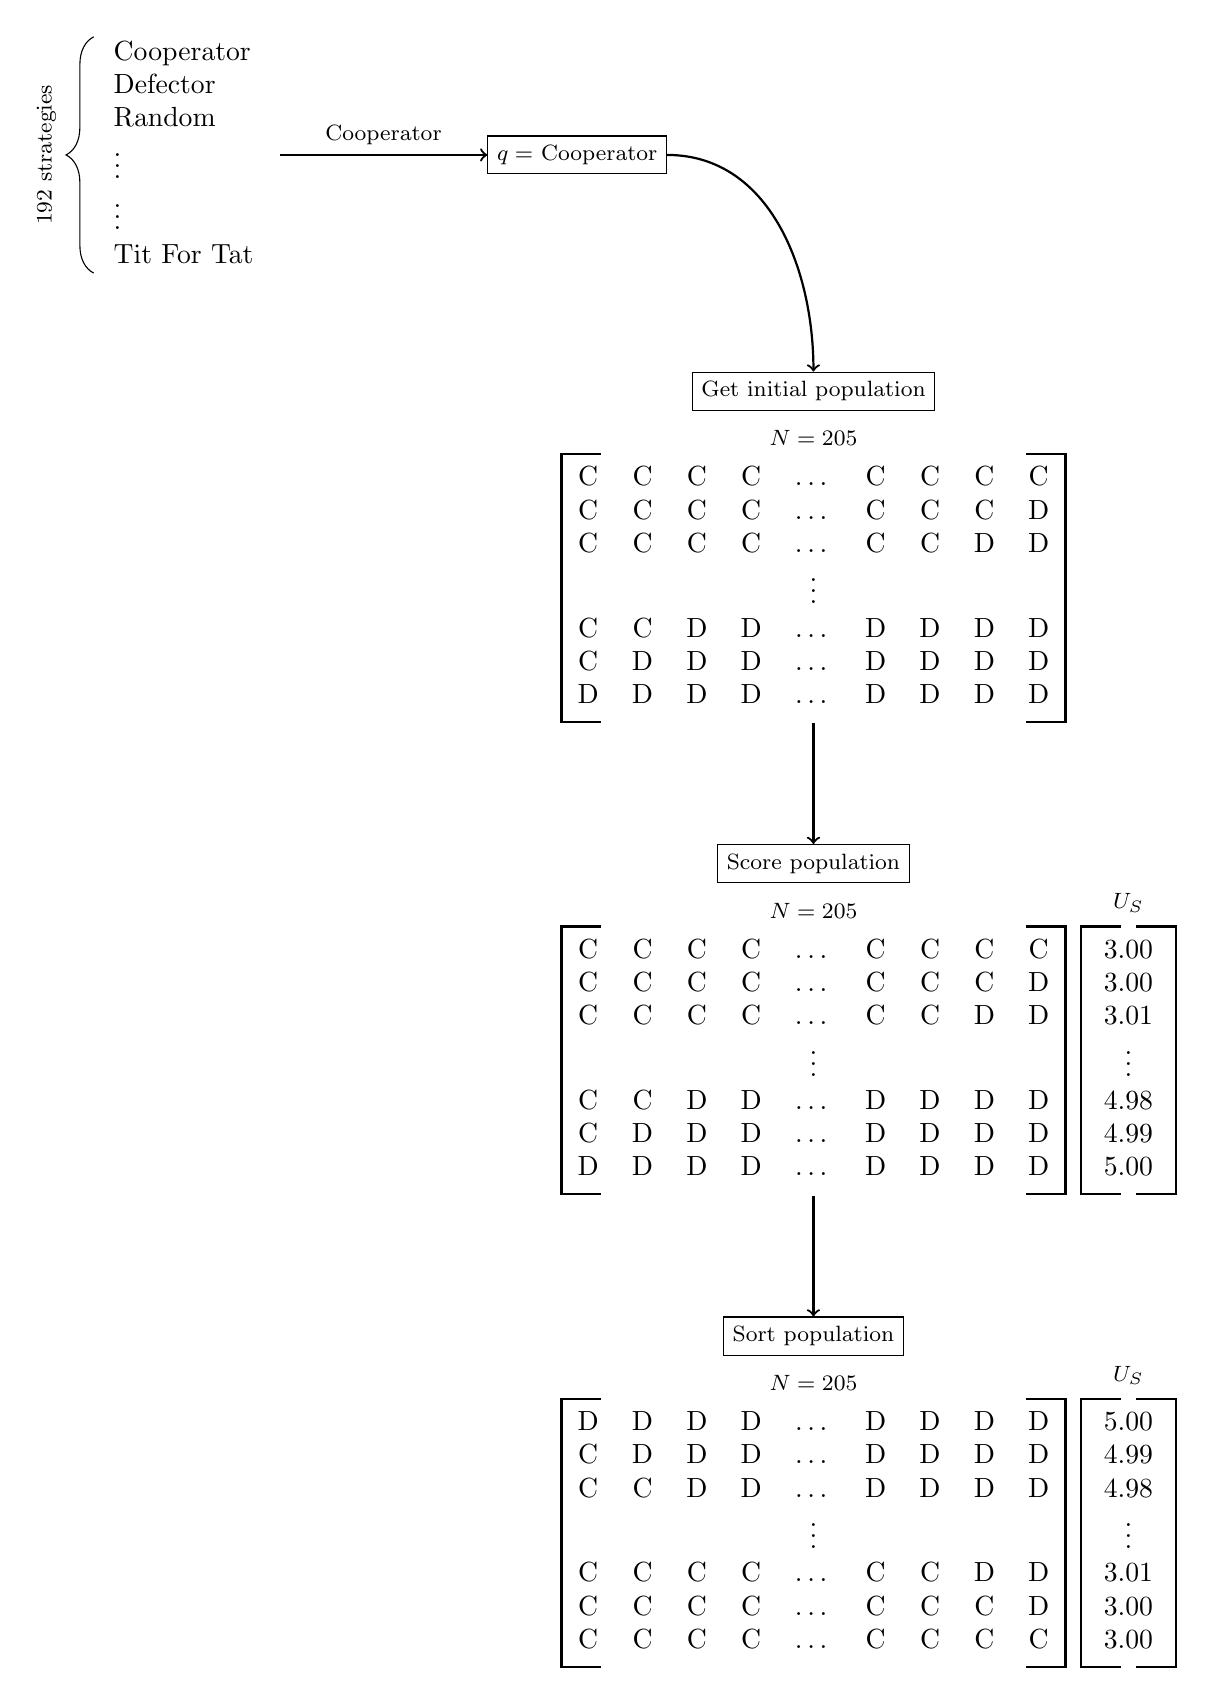
\begin{tikzpicture}

    \node (strategies) {
        \begin{tabular}{l}
            Cooperator \\
            Defector \\
            Random \\
            $\vdots$ \\
            $\vdots$ \\
            Tit For Tat
        \end{tabular}
    };
    
    \draw [decorate,decoration={brace,amplitude=10pt}, xshift=-4pt,yshift=0pt]
    (-1, -1.5) -- (-1, 1.5) node [black,midway,xshift=-0.6cm, rotate=90]
    {\footnotesize 192 strategies};

    % \node (point) at ($(strategies)+(4, 0)$) {};
    
    \node[draw=black] (opponent) at ($(strategies)+(5, 0)$) {\footnotesize \(q=\) Cooperator};
    \draw (strategies) edge[out=0, in=180, ->, thick] node [above] {\footnotesize Cooperator} (opponent);
    
    \node[draw=black] (init) at ($(opponent)+(3, -3)$) {\footnotesize Get initial population};
    \node (n) at ($(opponent)+(3, -3.6)$) {\footnotesize \(N=205\)};
    \node (initial_pop) at ($(opponent)+(3, -5.5)$) {\begin{tabular}{ccccccccc}
        C & C & C & C & \dots & C & C & C & C \\
        C & C & C & C & \dots & C & C & C & D \\
        C & C & C & C & \dots & C & C & D & D \\
        &&&& \(\vdots\) &&&& \\
        C & C & D & D & \dots & D & D & D & D \\
        C & D & D & D & \dots & D & D & D & D \\
        D & D & D & D & \dots & D & D & D & D \\
        \end{tabular}
     };
     \draw [black, thick] ($(initial_pop)+(-2.7, -1.7)$) to [square left brace ] ($(initial_pop)+(-2.7, 1.7)$);
     \draw [black, thick] ($(initial_pop)+(2.7, -1.7)$) to [square right brace] ($(initial_pop)+(2.7, 1.7)$);

    \draw (opponent) edge[out=-0, in=90, ->, thick] node {} (init);

    \node[draw=black] (init) at ($(initial_pop)+(0, -3.5)$) {\footnotesize Score population};
    \node (n) at ($(initial_pop)+(0, -4.1)$) {\footnotesize \(N=205\)};
    \node (score_population) at ($(initial_pop)+(0, -6)$) {\begin{tabular}{ccccccccc}
        C & C & C & C & \dots & C & C & C & C \\
        C & C & C & C & \dots & C & C & C & D \\
        C & C & C & C & \dots & C & C & D & D \\
        &&&& \(\vdots\) &&&& \\
        C & C & D & D & \dots & D & D & D & D \\
        C & D & D & D & \dots & D & D & D & D \\
        D & D & D & D & \dots & D & D & D & D \\
        \end{tabular}
     };

     \draw [black, thick] ($(score_population)+(-2.7, -1.7)$) to [square left brace ] ($(score_population)+(-2.7, 1.7)$);
     \draw [black, thick] ($(score_population)+(2.7, -1.7)$) to [square right brace]  ($(score_population)+(2.7, 1.7)$);

    \node (u) at ($(n)+(4, .1)$) {\footnotesize \(U_S\)};
    \node (score) at ($(score_population)+(4, 0)$) {\begin{tabular}{c}
        3.00 \\
        3.00 \\
        3.01 \\
        \(\vdots\)\\
        4.98 \\
        4.99 \\
        5.00 \\
        \end{tabular}
    };
     \draw [black, thick] ($(score)+(-.1, -1.7)$) to [square left brace ] ($(score)+(-.1, 1.7)$);
     \draw [black, thick] ($(score)+(.1, -1.7)$) to [square right brace] ($(score)+(.1, 1.7)$);

     \draw (initial_pop) edge[out=-90, in=90, ->, thick] (init);


     \node[draw=black] (init) at ($(score_population)+(0, -3.5)$) {\footnotesize Sort population};
     \node (n) at ($(score_population)+(0, -4.1)$) {\footnotesize \(N=205\)};
     \node (sort_population) at ($(score_population)+(0, -6)$) {\begin{tabular}{ccccccccc}
         D & D & D & D & \dots & D & D & D & D \\
         C & D & D & D & \dots & D & D & D & D \\
         C & C & D & D & \dots & D & D & D & D \\
         &&&& \(\vdots\) &&&& \\
         C & C & C & C & \dots & C & C & D & D \\
         C & C & C & C & \dots & C & C & C & D \\
         C & C & C & C & \dots & C & C & C & C \\
         \end{tabular}
      };
 
      \draw [black, thick] ($(sort_population)+(-2.7, -1.7)$) to [square left brace ] ($(sort_population)+(-2.7, 1.7)$);
      \draw [black, thick] ($(sort_population)+(2.7, -1.7)$) to [square right brace]  ($(sort_population)+(2.7, 1.7)$);
 
     \node (u) at ($(n)+(4, .1)$) {\footnotesize \(U_S\)};
     \node (score) at ($(sort_population)+(4, 0)$) {\begin{tabular}{c}
         5.00 \\
         4.99 \\
         4.98 \\
         \(\vdots\)\\
         3.01 \\
         3.00 \\
         3.00 \\
         \end{tabular}
     };
      \draw [black, thick] ($(score)+(-.1, -1.7)$) to [square left brace ] ($(score)+(-.1, 1.7)$);
      \draw [black, thick] ($(score)+(.1, -1.7)$) to [square right brace] ($(score)+(.1, 1.7)$);
 
      \draw (score_population) edge[out=-90, in=90, ->, thick] (init);
    \end{tikzpicture}
\end{document}